\documentclass[11pt, a4paper] {ncc}
\usepackage[utf8] {inputenc}
\usepackage[T2A]{fontenc}
\usepackage[english, russian] {babel}
\usepackage[usenames,dvipsnames]{xcolor}
\usepackage{listings,a4wide,longtable,amsmath,amsfonts,graphicx,tikz}
\usepackage{pgfplots}
\usepackage{indentfirst}
\usepackage{bytefield}

\lstdefinelanguage[8051]{Assembler}{
        keywords={cseg, at, mov, anl, dec, orl, jb, ljmp, end, acall, ret,
                  reti},
        comment=[l]{;},
        sensitive=false
}

\begin{document}
\frenchspacing
\pagestyle{empty}
% ============================ ТИТУЛЬНЫЙ ЛИСТ ================================
\begin{center}
     Национальный исследовательский университет информационных технологий,
                              механики и оптики\\
\vspace{\stretch{1}}
                        Кафедра вычислительной техники\\
                                Организация ЭВМ
\end{center}
\vspace{\stretch{2}}
\begin{center}
                               Курсовая работа\\
                          <<Проектирование микроЭВМ>>\\
                                Вариант 8
\end{center}
\vspace{\stretch{3}}
\begin{flushright}
                                                        Студенты: \\
                                                            {\it Куклина М., \\
                                                            Кириллова А., \\
                                                            гр. P3301} \\
                                                        Преподаватель: \\
                                                        {\it Скорубский В.И.}
\end{flushright}
\vspace{\stretch{4}}
\begin{center}
                                      Санкт-Петербург, 2017
\end{center}
\newpage
% ======================== КОНЕЦ ТИТУЛЬНОГО ЛИСТА ============================

% ================================ ОТЧЁТ =====================================

\section{Цель работы}
Целью курсового проекта является разработка микропрограммного управления и схемы ЭВМ с архитектурой
CISC и системой команд микроЭВМ (микрокомпьютер, MCU) MCS51.  Исходными данными являются программная
модель на уровне Ассемблера, перечень команд, выполняемых схемой.   
Для функционального описания микропрограмм и моделирования могут быть использованы языки программирования,
наиболее близким  из которых является язык Си в системе BorlandC++.     


\section{Система команд}

\subsection{\tt dec @rj}
\begin{bytefield}[bitwidth=2.2em]{8}
        \bitbox{1}{\color{lightgray}C}   &
        \bitbox{1}{\color{lightgray}AC}  &
        \bitbox{1}{\color{lightgray}F0}  &
        \bitbox{1}{\color{lightgray}RS1} &
        \bitbox{1}{\color{lightgray}RS0} &
        \bitbox{1}{\color{lightgray}OV}  &
        \bitbox{1}{\color{lightgray}~}   &
        \bitbox{1}{\color{lightgray}P}
\end{bytefield}

Команда записывает в ячейку памяти, адрес которой указан в регистре $R_i$,
значение, на единицу меньшее текущего.

\begin{description}
        \item[Размер] 1 байт
        \item[Число циклов] 1
        \item[Кодирование]~\\
                \begin{bytefield}[bitwidth=1.2em]{8}
                        \bitboxes*{1}{0000011i}
                \end{bytefield}
        \item[Алгоритм] $(R_i) \leftarrow (R_i) - 1$
        \item[Пример] \texttt{DEC @R0}
\end{description}
\hrulefill

\subsection{\tt dec a}
\begin{bytefield}[bitwidth=2.2em]{8}
        \bitbox{1}{\color{lightgray}C}   &
        \bitbox{1}{\color{lightgray}AC}  &
        \bitbox{1}{\color{lightgray}F0}  &
        \bitbox{1}{\color{lightgray}RS1} &
        \bitbox{1}{\color{lightgray}RS0} &
        \bitbox{1}{\color{lightgray}OV}  &
        \bitbox{1}{\color{lightgray}~}   &
        \bitbox{1}{\bf         P}
\end{bytefield}

Команда записывает в аккумулятор $a$ значение, на единицу меньшее текущего.

\begin{description}
        \item[Размер] 1 байт
        \item[Число циклов] 1
        \item[Кодирование]~\\
                \begin{bytefield}[bitwidth=1.2em]{8}
                        \bitboxes*{1}{00010100}
                \end{bytefield}
        \item[Алгоритм] $A \leftarrow A - 1$
        \item[Пример] \texttt{DEC A}
\end{description}
\hrulefill

\subsection{\tt orl c, bit}
\begin{bytefield}[bitwidth=2.2em]{8}
        \bitbox{1}{\bf         C}   &
        \bitbox{1}{\color{lightgray}AC}  &
        \bitbox{1}{\color{lightgray}F0}  &
        \bitbox{1}{\color{lightgray}RS1} &
        \bitbox{1}{\color{lightgray}RS0} &
        \bitbox{1}{\color{lightgray}OV}  &
        \bitbox{1}{\color{lightgray}~}   &
        \bitbox{1}{\color{lightgray}P}
\end{bytefield}

Команда считывает бит, адрес которого указан в операнде \texttt{bit}, и
записывает в $C$ результат логического сложения $C$ с этим битом.

\begin{description}
        \item[Размер] 2 байт
        \item[Число циклов] 2
        \item[Кодирование]~\\
                \begin{bytefield}[bitwidth=1.2em]{16}
                        \bitboxes*{1}{01110010} &
                                \bitbox{8}{bit\strut}
                \end{bytefield}
        \item[Алгоритм] $C \leftarrow C \lor b$
        \item[Пример] \texttt{ORL C, 22h}
\end{description}
\hrulefill

\subsection{\tt orl c, /bit}
\begin{bytefield}[bitwidth=2.2em]{8}
        \bitbox{1}{\bf         C}   &
        \bitbox{1}{\color{lightgray}AC}  &
        \bitbox{1}{\color{lightgray}F0}  &
        \bitbox{1}{\color{lightgray}RS1} &
        \bitbox{1}{\color{lightgray}RS0} &
        \bitbox{1}{\color{lightgray}OV}  &
        \bitbox{1}{\color{lightgray}~}   &
        \bitbox{1}{\color{lightgray}P}
\end{bytefield}

Команда считывает бит, адрес которого указан в операнде \texttt{bit}, и
записывает в $C$ результат логического сложения $C$ с битом, инверсным данному.

\begin{description}
        \item[Размер] 2 байт
        \item[Число циклов] 2
        \item[Кодирование]~\\
                \begin{bytefield}[bitwidth=1.2em]{16}
                        \bitboxes*{1}{10100000} &
                                \bitbox{8}{bit\strut}
                \end{bytefield}
        \item[Алгоритм] $C \leftarrow C \lor \neg b$
        \item[Пример] \texttt{ORL C, /22h}
\end{description}
\hrulefill

\subsection{\tt mov a, @rj}
\begin{bytefield}[bitwidth=2.2em]{8}
        \bitbox{1}{\color{lightgray}C}   &
        \bitbox{1}{\color{lightgray}AC}  &
        \bitbox{1}{\color{lightgray}F0}  &
        \bitbox{1}{\color{lightgray}RS1} &
        \bitbox{1}{\color{lightgray}RS0} &
        \bitbox{1}{\color{lightgray}OV}  &
        \bitbox{1}{\color{lightgray}~}   &
        \bitbox{1}{\bf         P}
\end{bytefield}

Команда записывает в аккумулятор $a$ содержимое ячейки памяти, адрес которой
указан в регистре $R_i$.

\begin{description}
        \item[Размер] 1 байт
        \item[Число циклов] 1
        \item[Кодирование]~\\
                \begin{bytefield}[bitwidth=1.2em]{8}
                        \bitboxes*{1}{1110011i}
                \end{bytefield}
        \item[Алгоритм] $A \leftarrow (R_i)$
        \item[Пример] \texttt{MOV A, @R1}
\end{description}
\hrulefill

\subsection{\tt mov a, ad}
\begin{bytefield}[bitwidth=2.2em]{8}
        \bitbox{1}{\color{lightgray}C}   &
        \bitbox{1}{\color{lightgray}AC}  &
        \bitbox{1}{\color{lightgray}F0}  &
        \bitbox{1}{\color{lightgray}RS1} &
        \bitbox{1}{\color{lightgray}RS0} &
        \bitbox{1}{\color{lightgray}OV}  &
        \bitbox{1}{\color{lightgray}~}   &
        \bitbox{1}{\bf         P}
\end{bytefield}

Команда записывает в аккумулятор $a$ содержимое ячейки памяти по адресу
\texttt{ad}.

\begin{description}
        \item[Размер] 2 байт
        \item[Число циклов] 1
        \item[Кодирование]~\\
                \begin{bytefield}[bitwidth=1.2em]{16}
                        \bitboxes*{1}{11100101} &
                                \bitbox{8}{ad\strut}
                \end{bytefield}
        \item[Алгоритм] $A \leftarrow (\text{ad})$
        \item[Пример] \texttt{MOV A, P0}
\end{description}
\hrulefill

\subsection{\tt jb bit, rel}
\begin{bytefield}[bitwidth=2.2em]{8}
        \bitbox{1}{\color{lightgray}C}   &
        \bitbox{1}{\color{lightgray}AC}  &
        \bitbox{1}{\color{lightgray}F0}  &
        \bitbox{1}{\color{lightgray}RS1} &
        \bitbox{1}{\color{lightgray}RS0} &
        \bitbox{1}{\color{lightgray}OV}  &
        \bitbox{1}{\color{lightgray}~}   &
        \bitbox{1}{\color{lightgray}P}
\end{bytefield}

Команда считывает бит \texttt{bit} и, если он установлен, переходит к адресу,
указанному во втором операнде.

\begin{description}
        \item[Размер] 3 байт
        \item[Число циклов] 2
        \item[Кодирование]~\\
                \begin{bytefield}[bitwidth=1.2em]{24}
                        \bitboxes*{1}{00100000} &
                                \bitbox{8}{bit\strut} &
                                \bitbox{8}{rel\strut}
                \end{bytefield}
        \item[Алгоритм] $\text{PC} \leftarrow \text{PC} + 3$\\
                $\text{IF}\ (\text{bit}) = 1,
                \text{PC} \leftarrow \text{PC} + \text{rel}$
        \item[Пример] \texttt{JB P1.2 LABEL}
\end{description}
\hrulefill

\section{Структура ЭВМ}

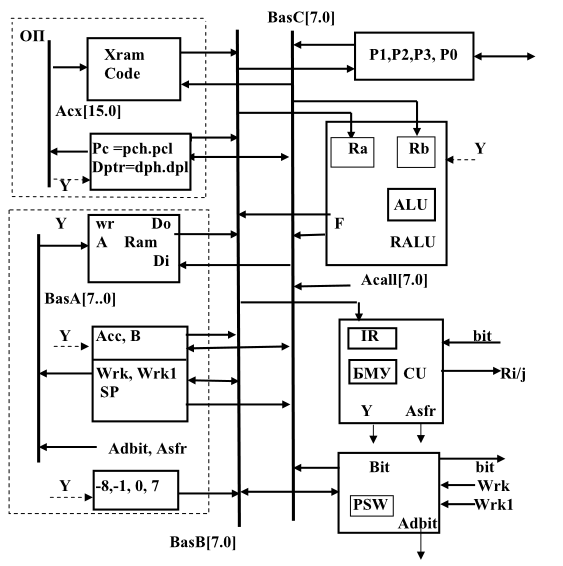
\includegraphics[width=0.8\textwidth]{evm.png}

\section{Функциональное тестирование}

\lstset{language=[8051]Assembler, tabsize=2}
\lstinputlisting{test.asm}

\section{Сниппеты изменений}

    \subsection{Формирование слова состояния \textbf{PSWC}}
        \begin{lstlisting}[language=C++]
    Q.printf("orlc "); 
    if (S == Q) {
        PSW |= (PB&(1 << (Wrk & 0x7))) ? 0x80 : 0x00;
    }
        \end{lstlisting}
    \subsection{\textbf{Button1Click}}

    Заполнение массива преобразования кода команды в адрес начала микрооперации.
        \begin{lstlisting}[language=C++]
    // dec @ri  : j = 9;
    for(uchar i = 0x16; i <= 0x17; ++i)
        ADC[i] = j;
    ++j;
    // dec a : j = 10;
    ADC[0x14] = j++;
    // orl c, bit : j = 11;
    ADC[0x72] = j++;
    // orl c, /bit : j = 12;
    ADC[0xA0] = j++;
    // mov a, @rj : j = 13;
    for(uchar i = 0xE6; i <= 0xE7; ++i)
        ADC[i] = j;
    ++j; 
    // mov ri, #d : j = 14;
    for(uchar i = 0x76; i <= 0x77; ++i)
        ADC[i] = j;
    ++j;
    // mov a, ad : j = 15;
    ADC[0xE5] = j++;
    // jb bit, rel : j = 16;
    ADC[0x20] = j++; 
    // mov ad, #d : j = 17;
    ADC[0x75] = j++;
        \end{lstlisting}

    Сброс и заполнение программной памяти.
        \begin{lstlisting}[language=C++]
 for (i = 0; i < 100; i++)
      CODE[i] = 0; // Reset
    PC = 0;
    //00: ljump 0x06
    CODE[PC++] = 0x02;
    CODE[PC++] = 0x00;
    CODE[PC++] = 0x04;
    //03: reti
    CODE[PC++] = 0x32;
    //04: mov 0xaa, #0x04
    CODE[PC++] = 0x75;
    CODE[PC++] = 0xaa;
    CODE[PC++] = 0x04;
    //07: mov a, 0xaa
    CODE[PC++] = 0xE5;
    CODE[PC++] = 0xaa;
    //09: dec a
    CODE[PC++] = 0x14;
    //0A: orl c, /ACC.1
    CODE[PC++] = 0xA0;
    CODE[PC++] = 0xE1;
    //0C: mov @r0, #0xaa
    CODE[PC++] = 0x77;
    CODE[PC++] = 0xaa;
    //0E: dec @r0
    CODE[PC++] = 0x17;
    //0F: mov a, @r0
    CODE[PC++] = 0xE7;
    //10: orl c, ACC.1
    CODE[PC++] = 0x72;
    CODE[PC++] = 0xE1;
    //12: jb Acc.1, ok ; true condition
    CODE[PC++] = 0x20;
    CODE[PC++] = 0xE1;
    CODE[PC++] = 0x03;
    //15: ljmp err
    CODE[PC++] = 0x02;
    CODE[PC++] = 0x00;
    CODE[PC++] = 0x15;
    //1b: jb acc.4, err ; false condition
    CODE[PC++] = 0x20;
    CODE[PC++] = 0xE4;
    CODE[PC++] = 0xfa;
    //1E: ljmp fin
    CODE[PC++] = 0x02;
    CODE[PC++] = 0x00;
    CODE[PC++] = 0x1b;
        \end{lstlisting}

    \subsection{Исполнение теста \textbf{Button2OnClick}}
        \begin{lstlisting}[language=C++]
      case 9: // dec @ri
      {
        { // 9.1. Read Ri (can only be R0 or R1)
          Wrk = Ram[(PSW & 0x18) | (IR & 0x1)];
          ss[0] = (IR & 0x1) | 0x30;
          ss[1] = '\0';
          char code[10] = "dec @r";
          Instr->Text = StrCat(code, ss);
        }
        { // 9.2. Read @Ri
          PB = Ram[Wrk] - 1;
        }
        { // 9.3. Write [@Ri - 1] to @Ri
          Ram[Wrk] = PB;
        }
        goto finish;
      }
      case 10: // dec a
      {
        { // 10.1. Modifying A
          Wrk = Ram[Acc] - 1;
        }
        { // 10.2. Writing A
          Ram[Acc] = ACC = Wrk;
          char code[12] = "dec a";
          ss[0] = '\0';
          Instr->Text = StrCat(code, ss);
        }
        { // 10.3. Updating the status register
          ss[0] = 'a';
          ss[1] = 'b';
          ss[2] = '\0';
          PSWC(ss);
          Ram[Psw] = PSW;
        }
        goto finish;
      }
      case 11: // orl c, bit
      {
        { // Reading the bit address
          Wrk = CODE[PC++];
          RAMK++;
          // Wrk = Ex = 1110 xxxx
          ss[0] = (Wrk & 0x0F) | 0x30;
          ss[1] = '\0';
          char code[12] = "orl c, Acc.";
          Instr->Text = StrCat(code, ss);
        }
        { // 7.2. Reading from SFR or RAM
          if (Wrk & 0x80)
            PB = Ram[Wrk & 0xf8];
          else
            PB = Ram[0x20 | ((Wrk & 0x78) >> 3)];
          RAMK++;
        }
        { // 7.3.
          PSWC("orlc ");
          RAMK++;
        }
        {
          Ram[Psw] = PSW;
          RAMK = 0;
        }
        goto finish;
      }
      case 12: // orl c, /bit
      {
        { // Reading the bit address
          Wrk = CODE[PC++];
          ss[0] = (Wrk & 0x7) | 0x30;
          ss[1] = '\0';
          char code[12] = "orl c, /";
          Instr->Text = StrCat(code, ss);
          RAMK++;
        }
        { // 7.2. Reading from SFR or RAM
          if (Wrk & 0x80)
            PB = Ram[Wrk & 0xf8];
          else
            PB = Ram[0x20 | ((Wrk & 0x78) >> 3)];
          PB = ~PB;
          RAMK++;
        }
        { // 7.3.
          PSWC("orlc ");
          RAMK++;
        }
        {
          Ram[Psw] = PSW;
          RAMK = 0;
        }
        goto finish;
      }
      case 13: // mov a, @rj
      {
        {
          Wrk = Ram[(PSW & 0x18) | (IR & 0x1)];
          RAMK++;
          ss[0] = (IR & 0x1) | 0x30;
          ss[1] = 0;
          char code[10] = "mov a,@r";
          Instr->Text = StrCat(code, ss);
        }
        {
          Ram[Acc] = ACC = Ram[Wrk];
          RAMK++;
          PSWC(ss); 
        }
        {
          Ram[Psw] = PSW;
          RAMK = 0;
        }

        goto finish;
      }
      case 14: // mov ri, #d
      {
        { // 14.1. Read Ri (can only be R0 or R1)
          /* Debug */ Wrk = CODE[PC++];
          Ram[(PSW & 0x18) | (IR & 0x1)] = Wrk;
          ss[0] = (IR & 0x1) | 0x30;
          ss[1] = '\0';
          char code[10] = "mov @r";
          Instr->Text = StrCat(code, ss);
        }
        goto finish;
      }
      case 15: // mov a, ad
      {
        {
          Wrk = CODE[PC++];
          RAMK++;
          itoa(Wrk, ss, 16);
          char code[10] = "mov a, ";
          Instr->Text = StrCat(code, ss);
        }
        {
          ACC = Ram[Wrk];
          RAMK++;
          PSWC(ss); 
        }
        { Ram[Acc] = ACC; }
        {
          Ram[Psw] = PSW;
          RAMK = 0;
        }

        goto finish;
      }
      case 16: // jb bit, rel
      {
        { // Reading the bit address
          Wrk = CODE[PC++];
        }
        {
          PA = CODE[PC++];
          RAMK++;
          ss[0] = (Wrk & 0x7) | 0x30;
          ss[1] = '\0';
          char code[12] = "jb Acc.";
          Instr->Text = StrCat(code, ss);
        }
        { // 7.2. Reading from SFR or RAM
          if (Wrk & 0x80)
            PB = Ram[Wrk & 0xF0];
          else
            PB = Ram[0x20 | ((Wrk & 0x78) >> 3)];
          RAMK++;
        }
        {
          char tmp = Wrk & 0x7;
          if (PB & (tmp & 0x1 ? tmp + 1 : tmp))
            PC += PA;
        }
        goto finish;
      }
      case 17: // mov ad, #d
      {
        {
          Wrk = CODE[PC++];
          RAMK++;
          itoa(Wrk, &ss[0], 16);
          char code[10] = "mov ad,#";
          Instr->Text = StrCat(code, ss);
        }
        {
          Ram[Wrk] = CODE[PC++];
          RAMK++;
        }
        goto finish;
      }
        \end{lstlisting}

	\section*{Вывод}
	В ходе выполнение курсовой работы изучалась архитектура micro51 и принципы проектирования и реализации ЭВМ.
    В результате выполнения работы были разработаны и интегрированы команды в соответствии с выданным вариантом.

\end{document}

